%!TEX program = xelatex
\documentclass[a4paper,fleqn,twocolumn]{article}
\usepackage{xeCJK}
\usepackage{geometry}
\geometry{left=2.0cm,right=2.0cm,top=2.5cm,bottom=2.5cm}
\usepackage{amsmath}
\usepackage{amssymb}
\usepackage{graphicx}
\usepackage{subcaption}
\newcommand{\di}[1]{\mathrm{d}#1}
\newcommand{\p}[2]{\frac{\partial #1}{\partial #2}}
\newcommand{\pp}[2]{\frac{\partial ^2 #1}{\partial #2 ^2}}
\newcommand{\dy}[2]{\frac{\di{#1}}{\di{#2}}}
\newcommand{\ddy}[2]{\frac{\mathrm{d} ^2 #1}{\mathrm{d} #2 ^2}}

\begin{document}
\section*{第二章}
    一、选择题\\
        1.C\par
        质点沿力方向位移为零。$\therefore A=0$.\\
        2.B\par
        $B$离开$A$时为弹簧恢复原长的时刻(该时刻之后,$A$受到弹簧拉力,加速度为负,$v_A<v_B$.)\par
        此时$v_A=v_B$.由动能定理:
        \begin{align*}
            \frac{1}{2}mv_A^2+\frac{1}{2}mv_B^2-0=\frac{1}{2}kd^2\\
            \therefore{}E_B=\frac{1}{2}mv_B^2=\frac{1}{4}kd^2
        \end{align*}
        3.C\par
        对$\vec{r}$求导:
        \begin{align*}
            \vec{v}&=\frac{\di{\vec{r}}}{\di{t}}\\
            &=-\frac{2\pi}{T}A\sin\frac{2\pi t}{T}\vec{i}+\frac{2\pi}{T}B\cos\frac{2\pi t}{T}\vec{j}
        \end{align*}
        \par$t=0$时,
        \begin{align*}
            v_1&=\sqrt{v_{x1}^2+v_{y1}^2}\\
            &=\sqrt{0^2+\left(\frac{2\pi}{T}B\right)^2}=\frac{2\pi}{T}B
        \end{align*}
        \[\therefore{}E_{k1}=\frac{1}{2}mv_1^2=\frac{2m\pi^2}{T^2}\left(B^2\right)\\\]
        \par$t=\frac{T}{4}$时,
        \begin{align*}
            v_2&=\sqrt{v_{x2}^2+v_{y2}^2}\\
            &=\sqrt{\left(-\frac{2\pi}{T}A\right)^2+0^2}=\frac{2\pi}{T}A
        \end{align*}
        \begin{gather*}
            \therefore{}E_{k2}=\frac{1}{2}mv_2^2=\frac{2m\pi^2}{T^2}\left(A^2\right)\\
            \therefore\Delta{}E_k=\frac{2\pi^2}{T^2}(B^2-A^2)
        \end{gather*}
        4.D\par
        由动量定理:
        \[0=m_1v_1-m_2v_2\]
        \[\therefore{}v_2=\frac{m_1}{m_2}v_1\]\par
        由机械能守恒:
        \begin{align*}
            E_p &=\frac{1}{2}m_1v_1^2+\frac{1}{2}m_2v_2^2\\
                &=\frac{m_1v_1^2+\frac{m_1^2v_1^2}{m_2}}{2}\\
                &=\frac{m_1v_1^2\left(m_1+m_2\right)}{2m_2}
        \end{align*}
        5.B\par
        (2):既然小车能在水平面上停止,说明水平面是粗糙的,有摩擦力做功。因此不满足机械能守恒。\par
        (4):重力做正功,摩擦力做负功,符号相反。\\
        6.D\par
        弹簧上任意一点弹力相同,记为N。截去一半后,伸长量缩短了一半,而弹力不变,因此k变为原来的两倍。\par
        并联在一起后,每一根弹簧受力为原先的一半。由$F=kA$,伸长量为原来的$\frac{1}{4}$。\par
        写成数学式子如下:
        \begin{align*}
            E_k &=2\times\left(\frac{1}{2}k'A'^2\right)\\
                &=\left(2k\right)\times\left(\frac{1}{4}A\right)^2\\
                &=\frac{1}{8}kA^2
        \end{align*}
        7.D\par 
        物体沿重力方向的位移为负,因此重力做负功。其它选项,物体沿推力方向有位移,因此推力做功,A错误;推力功与摩擦力做的功和重力做的功之和等值反号,因此BC错误。\\
        8.C\par 
        若合外力的冲量为0,则由冲量定义$\vec{I}=\int_{t1}^{t2}\vec{F}\di{t}$知,$\vec{F}=\vec{0}$,因此合外力做的功为0。其它选项,AD可举匀速圆周运动的反例;对于B,合外力不为0,必有加速度,而质量不改变,因此$\vec{v}$必然改变,即动量必改变。\\
        9.B\par 
        由动能表达式$E_k=\frac{p^2}{2m}$,在动量相同的情况下,质量越大,动能越小,因此选B\\
        10.A\par 
        设小球重力为$G$,弹簧弹性系数为$k$,则$G=kd$,再设最低点时弹簧伸长$h$。以弹簧原长的高度为基准,释放前和最低点为始末态,应用机械能守恒:
        \[Gh=\frac{1}{2}kh^2\]
        解得$h=2d$\\
    二、填空题\\
    	11.$31J$
    	\[A=\int_{0.5}^{1}F\di{x}=\int_{0.5}^{1}(52.8x+38.4x^2)\di{x}=31(J)\]
   		12.$24J$ $4m/s$\par 
   		\[A=\int_{1}^{4}F\di{x}=\int_{1}^{4}(3+2x)\di{x}=24(J)\]
   		\[\text{由动能定理:}\frac{1}{2}mv^2=24,\quad \therefore v=4(m/s)\]
   		13.$\frac{GMm}{6R}$ \qquad $-\frac{GMm}{3R}$
   		\begin{gather*}
   			\text{卫星运动的向心力由万有引力提供,}\therefore m\frac{v^2}{3R}=G\frac{Mm}{(3R)^2}\\
   			\therefore E_k=\frac{1}{2}mv^2=\frac{GMm}{6R}\\
   			\text{由引力势能公式:}E_p=-\frac{GMm}{r}=-\frac{GMm}{3R}
   		\end{gather*}
   		14.1296
   		\begin{gather*}
   			\text{由牛顿第二定律:}F=ma,\qquad t^2=2a=2\ddy{x}{t},\\
   			\text{再由初始条件}t=0,x=0\text{且}v=0, \text{解得}x=\frac{1}{24}t^4\\
   			\text{由此可知}x=54m\text{时}, t=6s\\
   			A=\int_{0}^{6}F\di{x}=\int_{0}^{6}t^2\di{(\frac{1}{24}t^4)}\\
   			\therefore A=1296J
   		\end{gather*}
   		15.$19.8m/s$\par
   		(小行星的物理量下标为1)
   		\begin{gather}
   			\text{向心力由万有引力提供,}\therefore m\frac{v_1^2}{R_1}=G\frac{Mm}{R_1^2}\notag\\
   			\text{将}M=\frac{4}{3}\pi R^3\rho\text{代入,得}v_1=\sqrt{G\frac{4}{3}\pi\rho R_1^2}\\
   			\text{由地球上重力为}g=9.8m/s,mg=G\frac{Mm}{R_2^2}\notag\\
   			\therefore g=G\frac{4}{3}\pi R_2\rho.\text{则}G\frac{4}{3}\pi\rho=\frac{g}{R_2}\notag\\
   			\text{代入(1),}v_1=\sqrt{\frac{gR_1^2}{R_2}}\approx19.8(m/s)\notag
   		\end{gather}
   		16.$\sqrt{\frac{2Mgh}{m+M}}$ \qquad $\frac{m^2gh}{M+m}$
   		\begin{gather}
   			\text{由动量定理:}mv_1=Mv_2\\
   			\text{由机械能守恒:}mgh=\frac{1}{2}mv_1^2+\frac{1}{2}Mv_2^2\\
   			\text{联立(1)(2)解得:}v_1=\sqrt{\frac{2Mgh}{m+M}}\notag\\
   			v_2=\sqrt{\frac{2m^2gh}{(m+M)M}}\notag\\
   			\text{由动能定理知,物块对滑道做的功就是滑道动能改变量}\notag\\
   			\text{即}\frac{1}{2}Mv_2^2=\frac{m^2gh}{M+m}\notag
   		\end{gather}
   		17.第i个质点所受合力做的功(类似说法均正确)\\
   		18.1m/s \qquad 200J\par
   		船员用200N的力拉绳子,由牛顿第三定律,绳子也给船员(和船)200N的拉力。以人和船为对象应用牛顿第二定律,解得:
   		\[a=\frac{F}{m}=0.5m/s^2\]
   		因此第2秒末速率为1m/s,增加的动能就是
   		\[E_k=\frac{1}{2}mv^2=\frac{1}{2}\times400\times1^2=200(J)\]
   		19.$\left(\frac{1}{r_2}-\frac{1}{r_1}\right)GMm$ 
   		\begin{gather*}
   			\text{由机械能守恒,}0+E_{p1}=E_k+E_{p2}\\
   			\therefore E_k=E_{p2}-E_{p1}=\left(\frac{1}{r_2}-\frac{1}{r_1}\right)\\
   			\text{以两个质点为系统,仅有万有引力(内力)做功,因此由质点系动能定理:}\\
   			A=E_k=\left(\frac{1}{r_2}-\frac{1}{r_1}\right)GMm
   		\end{gather*}
   		20.$0.8\sqrt{2}$\par
   		\centering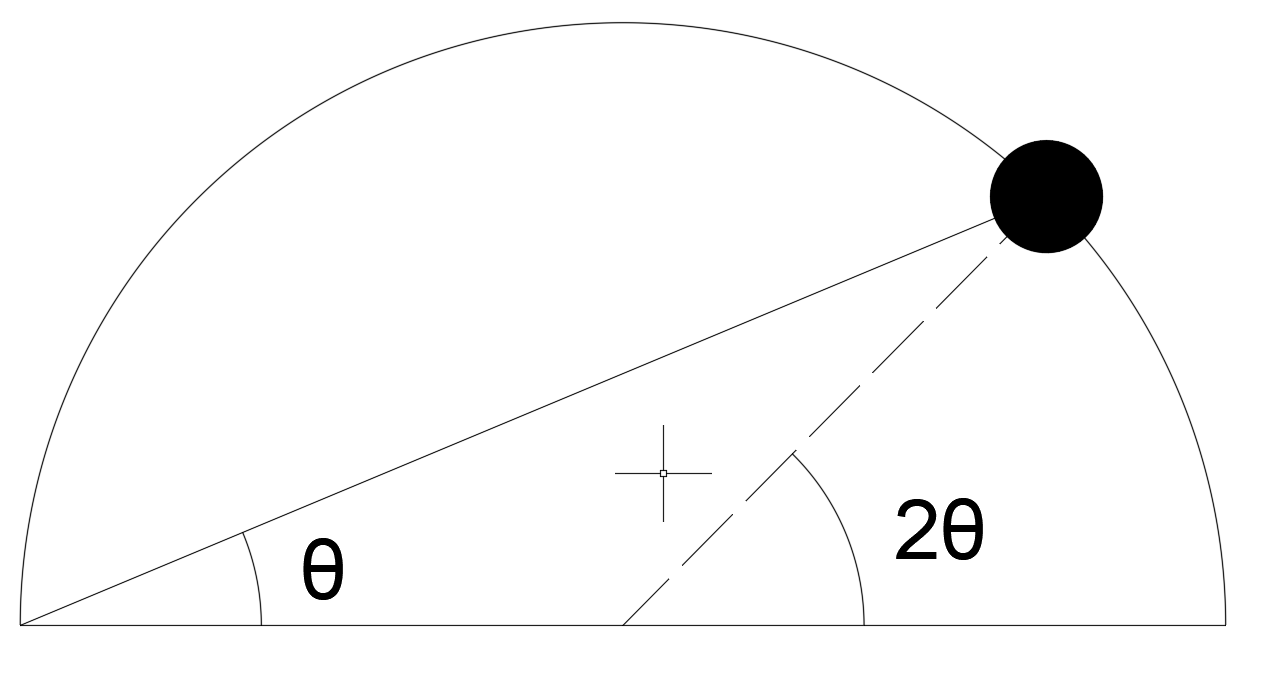
\includegraphics[height=100pt]{Chp2_illus1.png}\\
   		图1
   		\begin{align*}
   			A	&=\int_{\theta=0}^{\theta=\frac{\pi}{4}}{vec{F}}\cdot\di{vec{x}}\\
   				&=\int_{\theta=0}^{\theta=\frac{\pi}{4}}F\di{x}\cos\left(\frac{\pi}{2}-\theta\right)\\
   				&=\int_{0}^{\frac{\pi}{4}}k(2R\cos\theta-0.1)\times\di{(R\times 2\theta)}\times\sin\theta\\
   				&=\int_{0}^{\frac{\pi}{4}}(-4R^2k\cos\theta+0.2Rk)\di{(\cos\theta)}\\
   				&=-2R^2k\cos^2\theta+0.2Rk\cos\theta\left.\right|_0^{\frac{\pi}{4}}\\
   				&=-2\times 0.2^2\times 40\times({\frac{\sqrt{2}}{2}}^2-1^2)+0.2\times 0.2\times 40\times(\frac{1}{2}-1)\\
   				&=0.8\sqrt{2}
   		\end{align*}
   	\raggedright
   	三、计算题\\
   		21.(1)
   		\begin{gather*}
   			\Delta l=\frac{F}{k}\\
   			E_p=\frac{1}{2}k(\Delta l)^2=\frac{F^2}{2k}\\
   			\text{由机械能守恒,}E_{kright}-0=E_p-0\\
   			\therefore\frac{1}{2}Mv_{\text{右}}^2=\frac{F^2}{2k}\\
   			\therefore v_{\text{右}}=\frac{F}{\sqrt{Mk}}
   		\end{gather*}
   		(2)
   		\begin{gather*}
   			\text{由受力分析知,}a_{\text{左}}=a_{\text{右}},\quad\text{即}\dy{v_{\text{左}}}{t}=-\dy{v_{\text{右}}}{t}\\
   			\text{两边积分:}\therefore v_{\text{左}}=-v_{\text{右}}+c\\
   			\text{代入刚恢复原长时:}v_{\text{左}}=0,v_{\text{右}}=\frac{F}{\sqrt{Mk}}\\
   			\therefore v_{\text{左}}+v_{\text{右}}=\frac{F}{\sqrt{Mk}}\\
   			\therefore\text{当}v_{\text{左}}=v_{\text{右}}\text{时},v'_{\text{左}}=v'_{\text{右}}=\frac{F}{\sqrt{2Mk}}\\
   			\text{由机械能守恒:}\\
   			0+\frac{1}{2}M(v_{\text{右}})^2=\frac{1}{2}k(\Delta l)^2+\frac{1}{2}M(v'_{\text{左}})^2+\frac{1}{2}M(v'_{\text{右}})^2\\
   			\therefore\Delta l=\pm\sqrt{\frac{M\left(\frac{F^2}{Mk}-2\times\frac{F^2}{4Mk}\right)}{k}}\\
   			=\pm\frac{\sqrt{2}}{2}\frac{F}{k}\\
   			\text{即伸长或压缩}\frac{\sqrt{2}}{2}\frac{F}{k}
   		\end{gather*}
   		22.\par 
   			记x为链条右端的位移,l为桌边链条的长度。
   			\begin{align*}
   				dA	&=F\cdot\di{x}\\
   					&=F\di{x}
   			\end{align*}
   			链条被匀速拉起,可知$F=G$
   			\begin{align*}
   				F	&=G=M'g\\
   					&=\frac{l}{L}Mg
   			\end{align*}
   			由几何意义,$\di{x}=-\di{l}$
   			\begin{align*}
	   			\therefore A&=\int_{\frac{L}{3}}^{0} -\frac{l}{L}Mg\di{l}\\
	   						&=\frac{Mg}{2L}l^2\left.\right|_{0}^{\frac{L}{3}}\\
	   						&=\frac{MgL}{18}
   			\end{align*}
   			如果有摩擦力f,则
   			\begin{align*}
	   			\di{A}	&=F'\di{x}\\
	   			F'		&=G+f=\frac{l}{L}Mg+\mu\left(\frac{L-l}{L}Mg\right)\\
	   					&=\frac{Mg}{L}[\mu L+(1-\mu)l]\\
	   			\therefore A&=\int_{\frac{L}{3}}^{0} -\frac{Mg}{L}[\mu L+(1-\mu)l] \di{l}\\
	   						&=\frac{Mg}{L}\left(\mu Ll+\frac{1-\mu}{2}l^2\right)\left.\right|_{0}^{\frac{L}{3}}\\
	   						&=\frac{Mg}{L}\left(\frac{\mu}{3}L^2+\frac{1-\mu}{18}L^2\right)\\
	   						&=MgL\frac{5\mu +1}{18}
   			\end{align*}
   		23.\par
   		\centering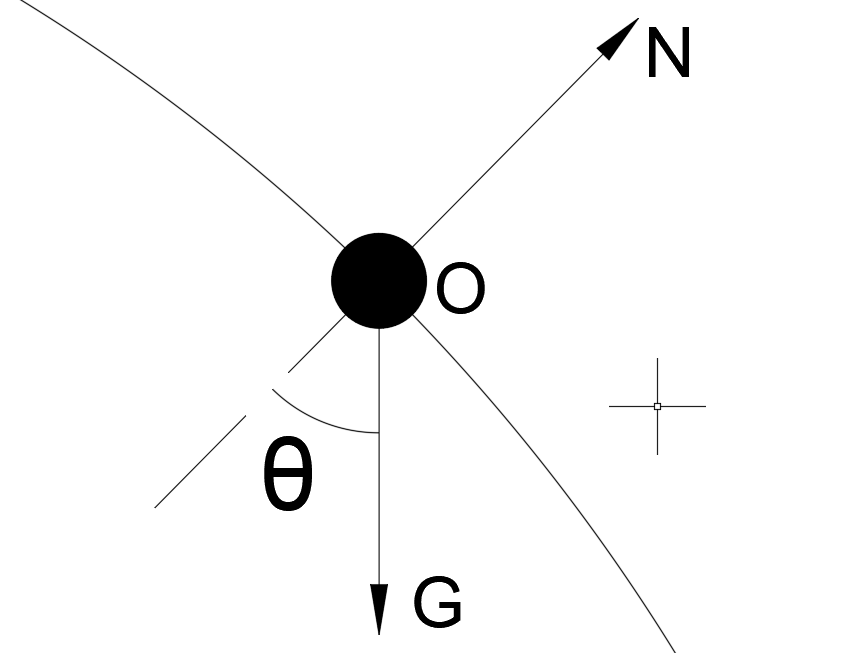
\includegraphics[height=100pt]{Chp2_illus2.png}\\
   		图2\\
   		\raggedright 由图2,对小球应用牛顿第二定律:
   		\[m\frac{v^2}{R}=mg\cos\theta-N\]
		\centering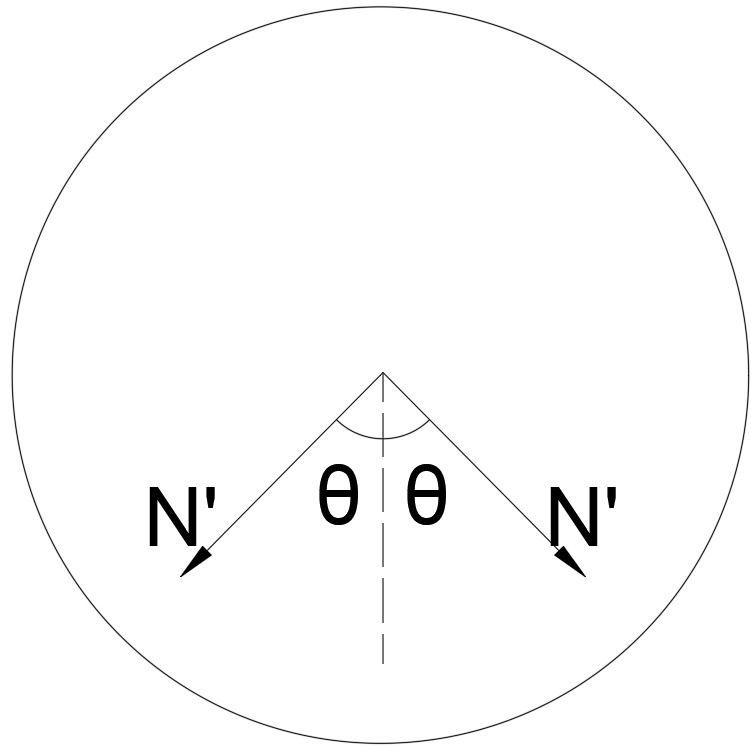
\includegraphics[height=100pt]{Chp2_illus3.png}\\
		图3\\
		\raggedright 由受力分析知,圆环竖直方向受力F为:
   		\begin{gather*}
   			F=(N'+N')\cos\theta=2N\cos\theta
   			\text{当}\theta\in[0,\frac{\pi}{2}]\text{时},\cos\theta>0\\
   			\therefore\text{当}N<0\text{时},F\text{向上,圆环上升}\\
   			\therefore N=mg\cos\theta-m\frac{v^2}{R}<0\\
   			\text{由机械能守恒(见图4):}\frac{1}{2}mv^2=mgh=mg(1-\cos\theta)R\\
   		\end{gather*}
   		\centering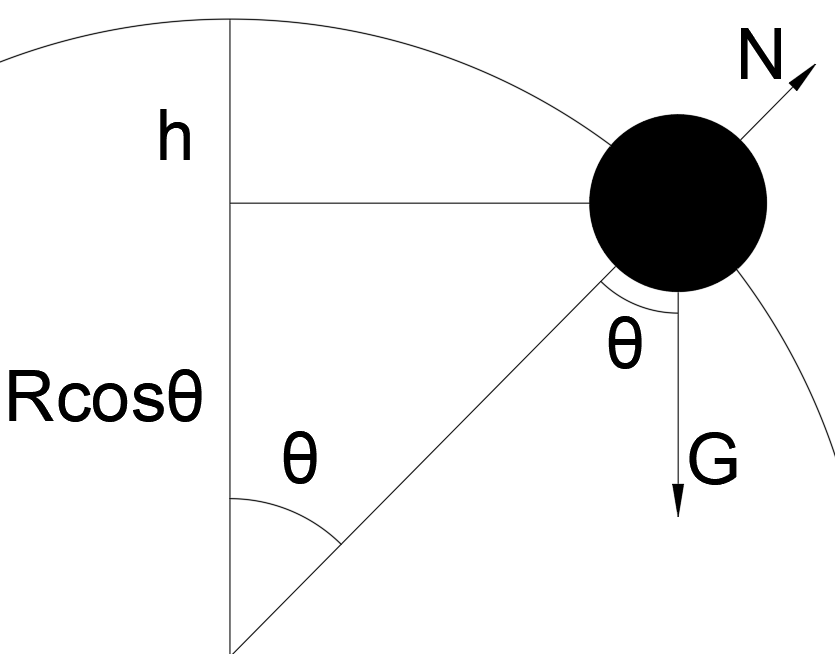
\includegraphics[height=100pt]{Chp2_illus4.png}\\
   		图4
   		\begin{gather*}
   			\text{代入,}\therefore mg\cos\theta-2mg(1-\cos\theta)<0\\
   			\therefore 3\cos\theta<2,\quad \theta>\arccos\frac{2}{3}\\
   			\text{即当}\theta>\arccos\frac{2}{3}\text{时,圆环会上升}
   		\end{gather*}
   		\raggedright
   		24.
   		\begin{gather*}
	   		T_1\text{提供}G1+G2\\
	   		\therefore k_1\Delta l=(m_1+m_2)g\\
	   		\Delta l=\frac{(m_1+m_2)g}{k_1}\\
	   		\text{由机械能守恒:}\\
	   		-mgx+\frac{1}{2}k_1(\Delta l+x)^2+\frac{1}{2}m_1v^2=0+\frac{1}{2}k_1(\Delta l)^2+0
	   	\end{gather*}
	   	\begin{align*}
	   		\therefore v&=\sqrt{\frac{-kx^2-2(k_1\Delta l-m_1g)x}{m_1}}\\
	   					&=\sqrt{-\frac{k_1}{m_1}x^2-\frac{2m_2g}{m_1}x}
	   	\end{align*}
	   	利用二次函数最大值为$\frac{4ac-b^2}{4a}$的性质:
	   	\begin{align*}
	   		v_{max}	&=\sqrt{\frac{0-\frac{4m_2^2g^2}{m_1^2}}{4\left(-\frac{k_1}{m_1}\right)}}\\
	   				&=\sqrt{\frac{m_2^2g^2}{m_1k_1}}=\frac{0.3\times 9.8}{\sqrt{0.5\times 8.9\times 10^4}}\\
	   				&=0.0139(m/s)
   		\end{align*}
\end{document}